\chapter{Results: Published Articles}
\chapterquote{Always pass on what you have learned.}{Yoda, Episode VIII}
\newpage

%% Section 1
\fakesection{Cain Triangle}\label{chap1}
\newpage

\subsection{Unraveling lipid and inflammation interplay in cancer, aging and infection for novel theranostic approaches}\label{art:lipids_review}
% \noindent
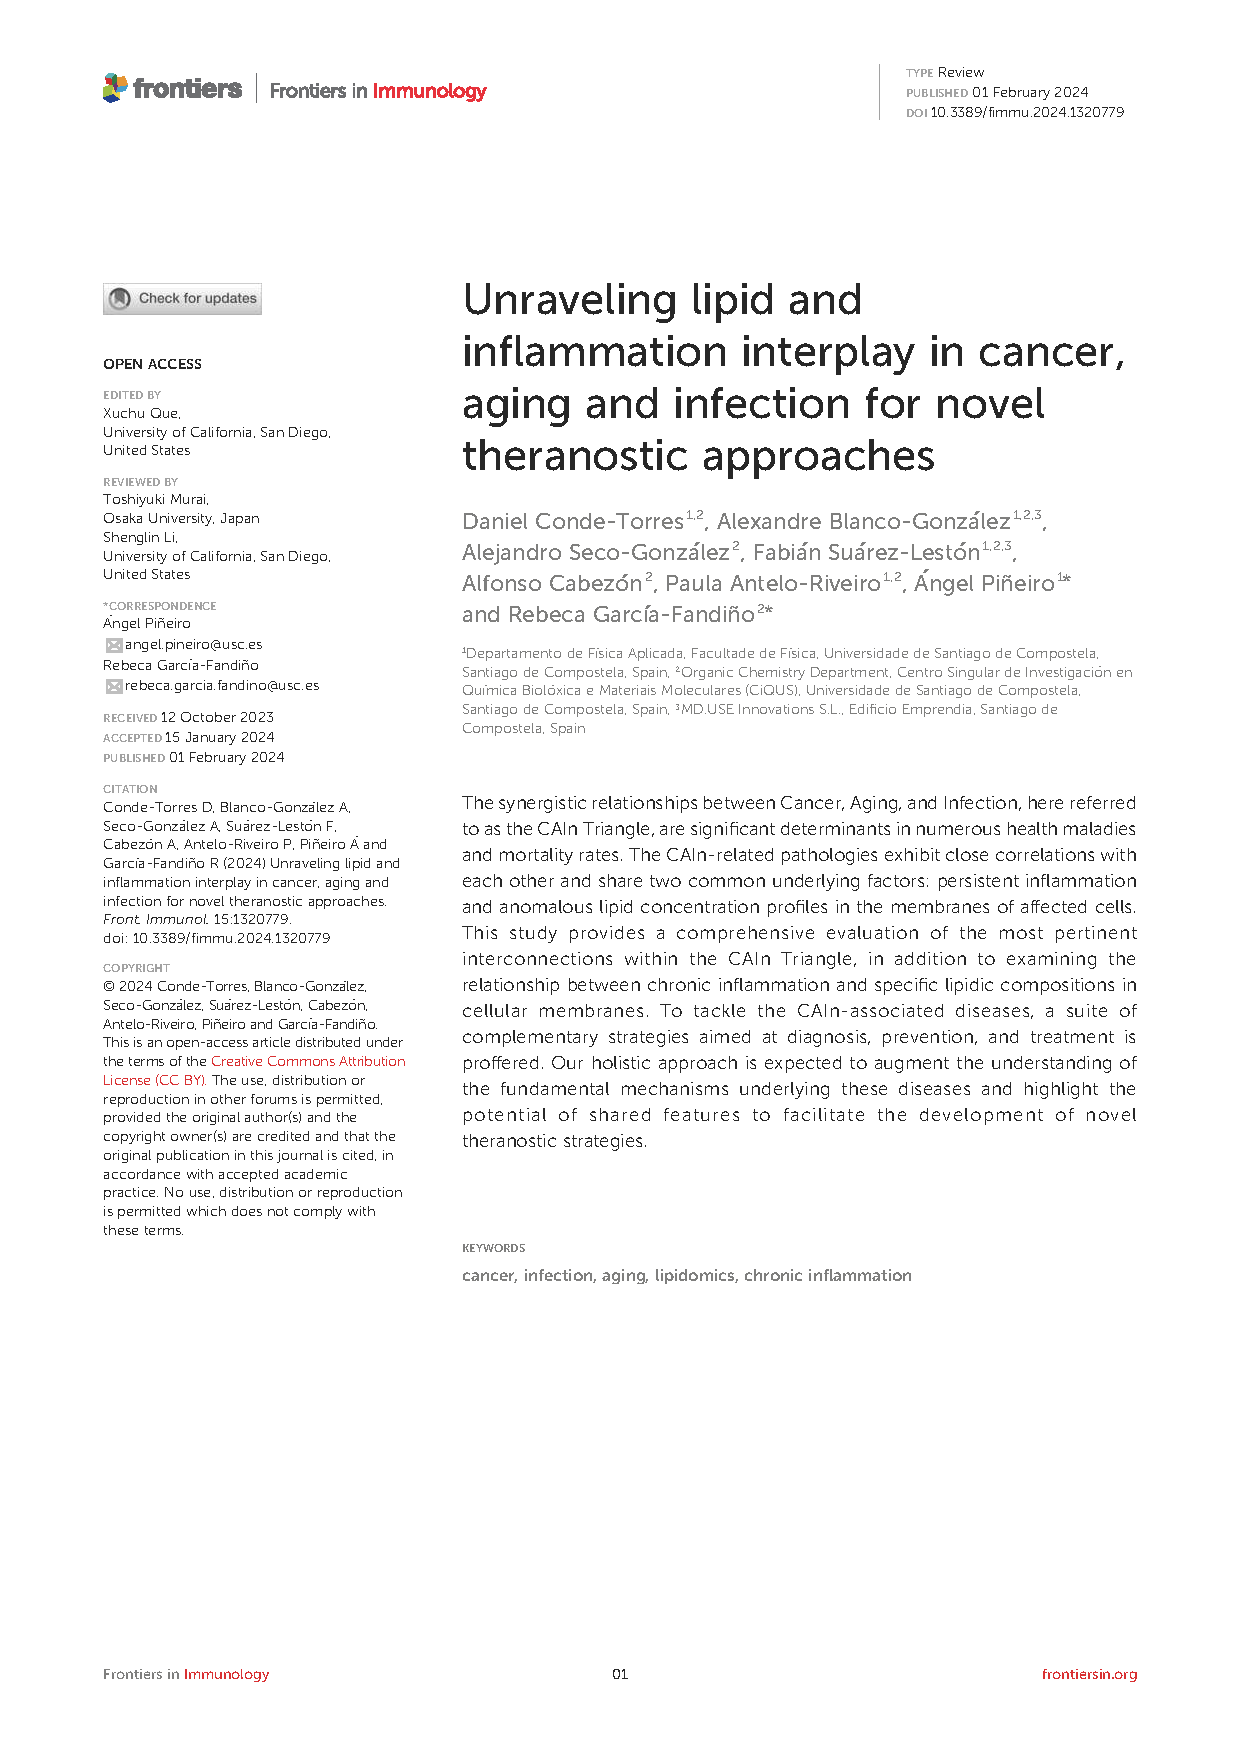
\includegraphics[page=1, width = 1.06\linewidth]{Results_Discussion/Papers/Papers_principales/Introduction_lipids_compressed.pdf}


\includepdf[pages=2-, width = 1.15\linewidth, pagecommand={\thispagestyle{fancy}}]{Results_Discussion/Papers/Papers_principales/Introduction_lipids_compressed.pdf}

%% Section 2
\fakesection{Metadynamics}\label{chap2}
\newpage

\subsection{Unlocking the specificity of antimicrobial peptide interactions for membrane-targeted therapies}\label{art:metadynamics}

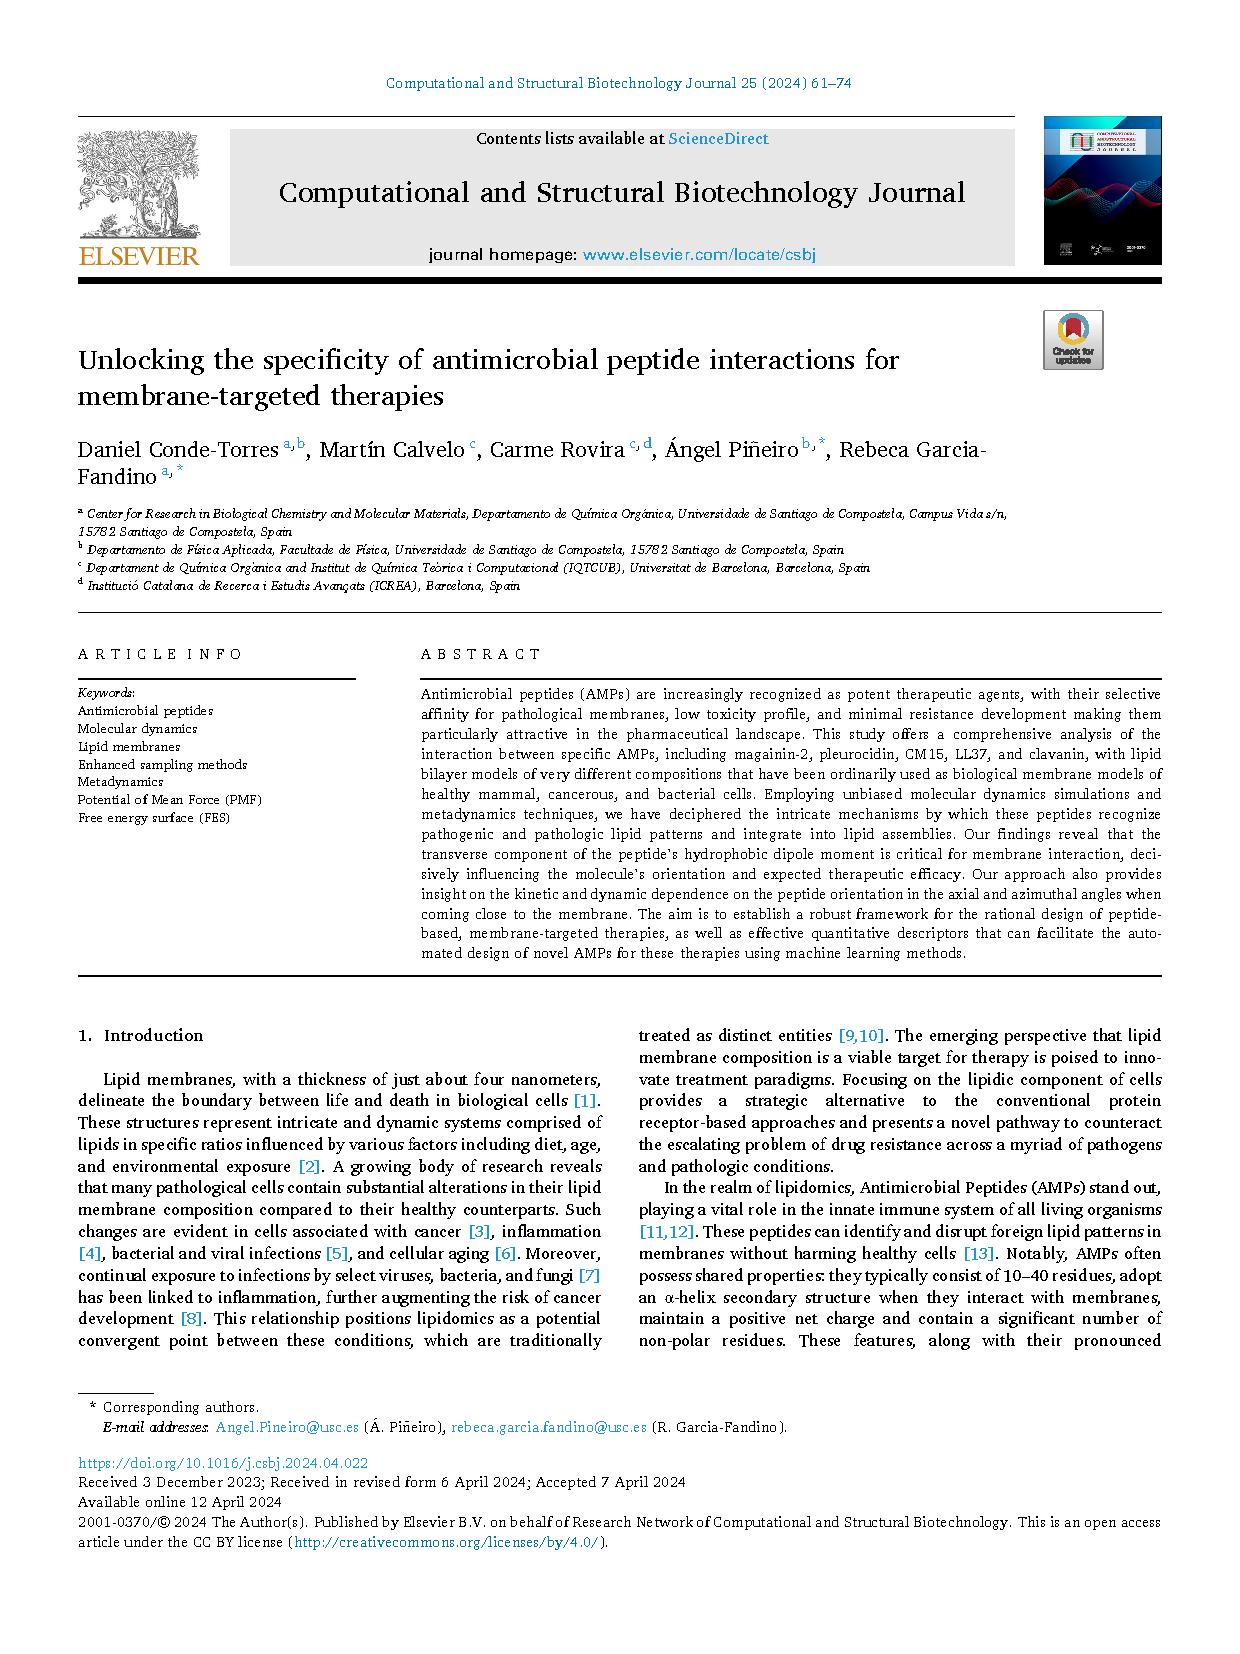
\includegraphics[page=1, width = \linewidth]{Results_Discussion/Papers/Papers_principales/metadinamica.pdf}


\includepdf[pages=2-, width = 1.2\linewidth, pagecommand={\thispagestyle{fancy}}]{Results_Discussion/Papers/Papers_principales/metadinamica.pdf}

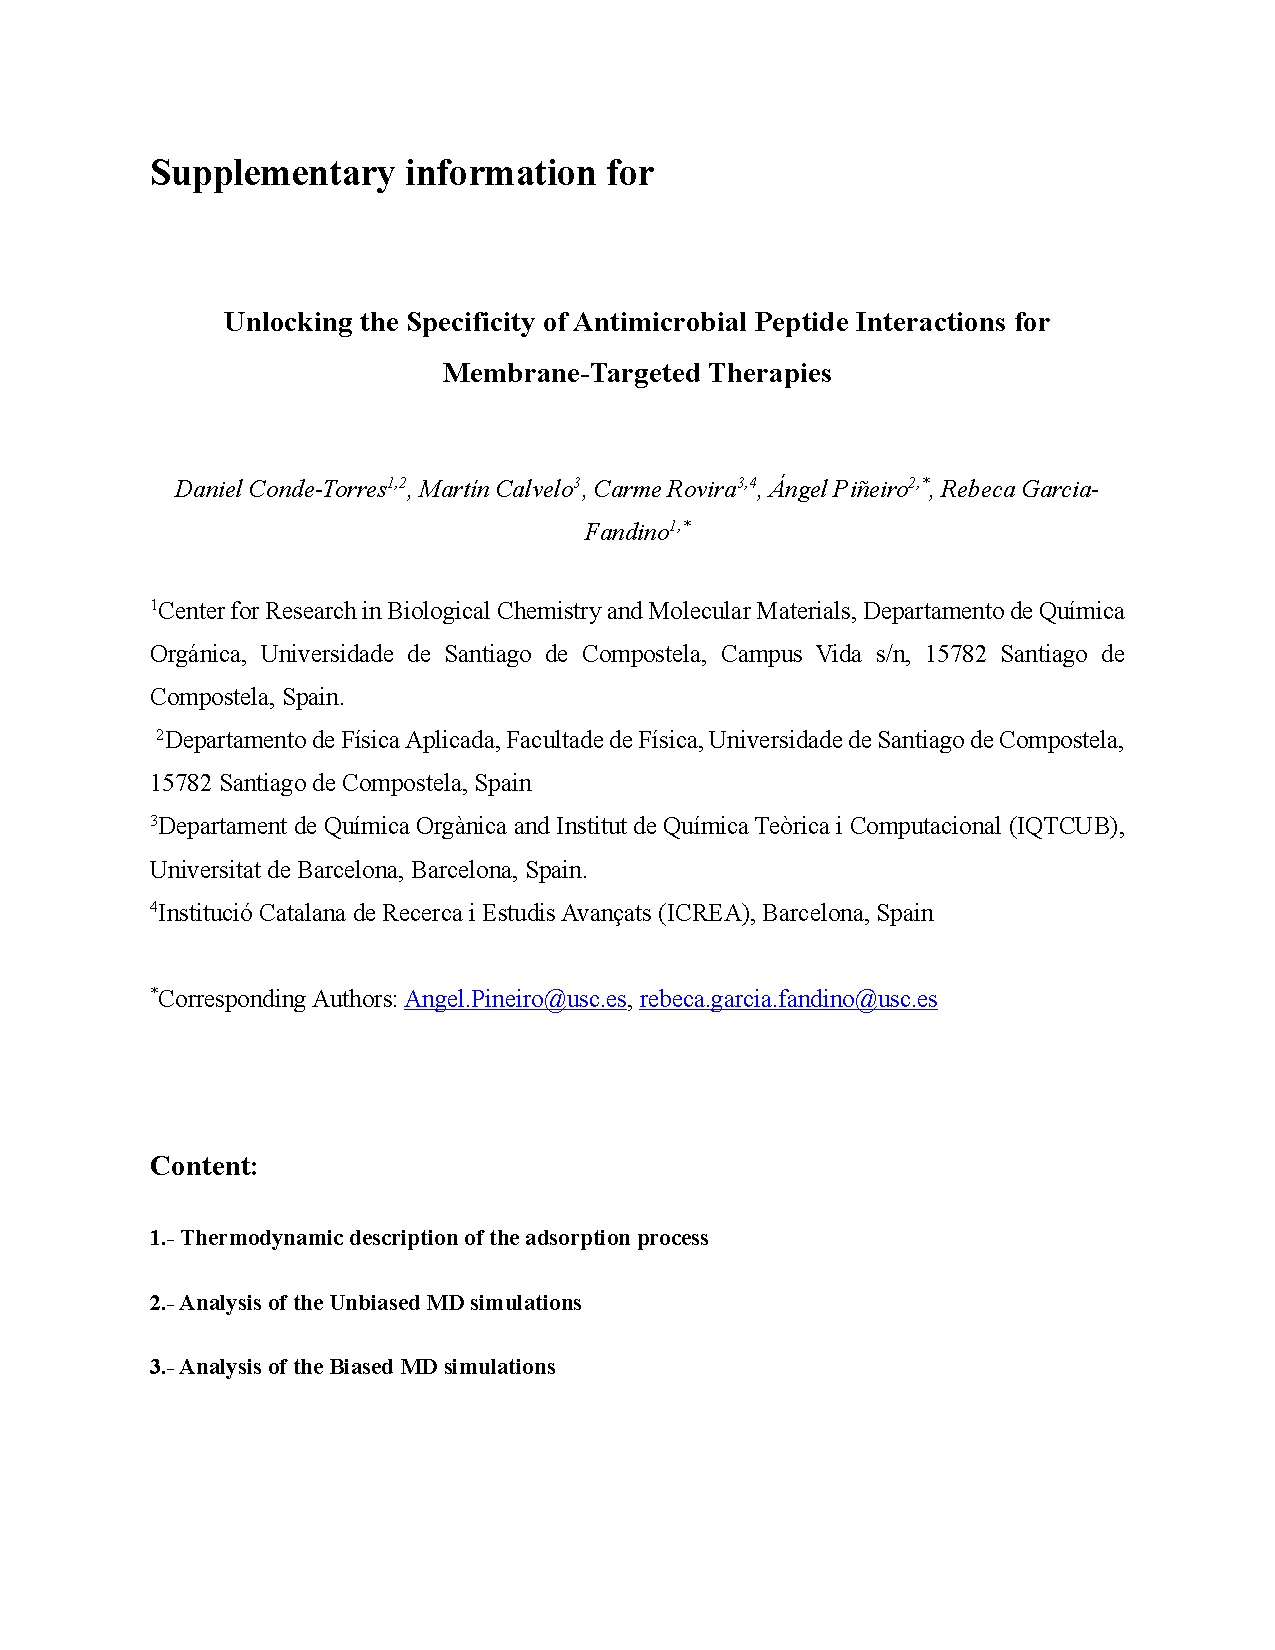
\includepdf[pages=1-, width = 1.2\linewidth, pagecommand={\thispagestyle{fancy}}]{Results_Discussion/Papers/Papers_principales/metadinamica_SI.pdf}


\subsection{Classical Simulations on Quantum Computers: Interface-Driven Peptide Folding on Simulated Membrane Surfaces}\label{art:vqe_cesga}

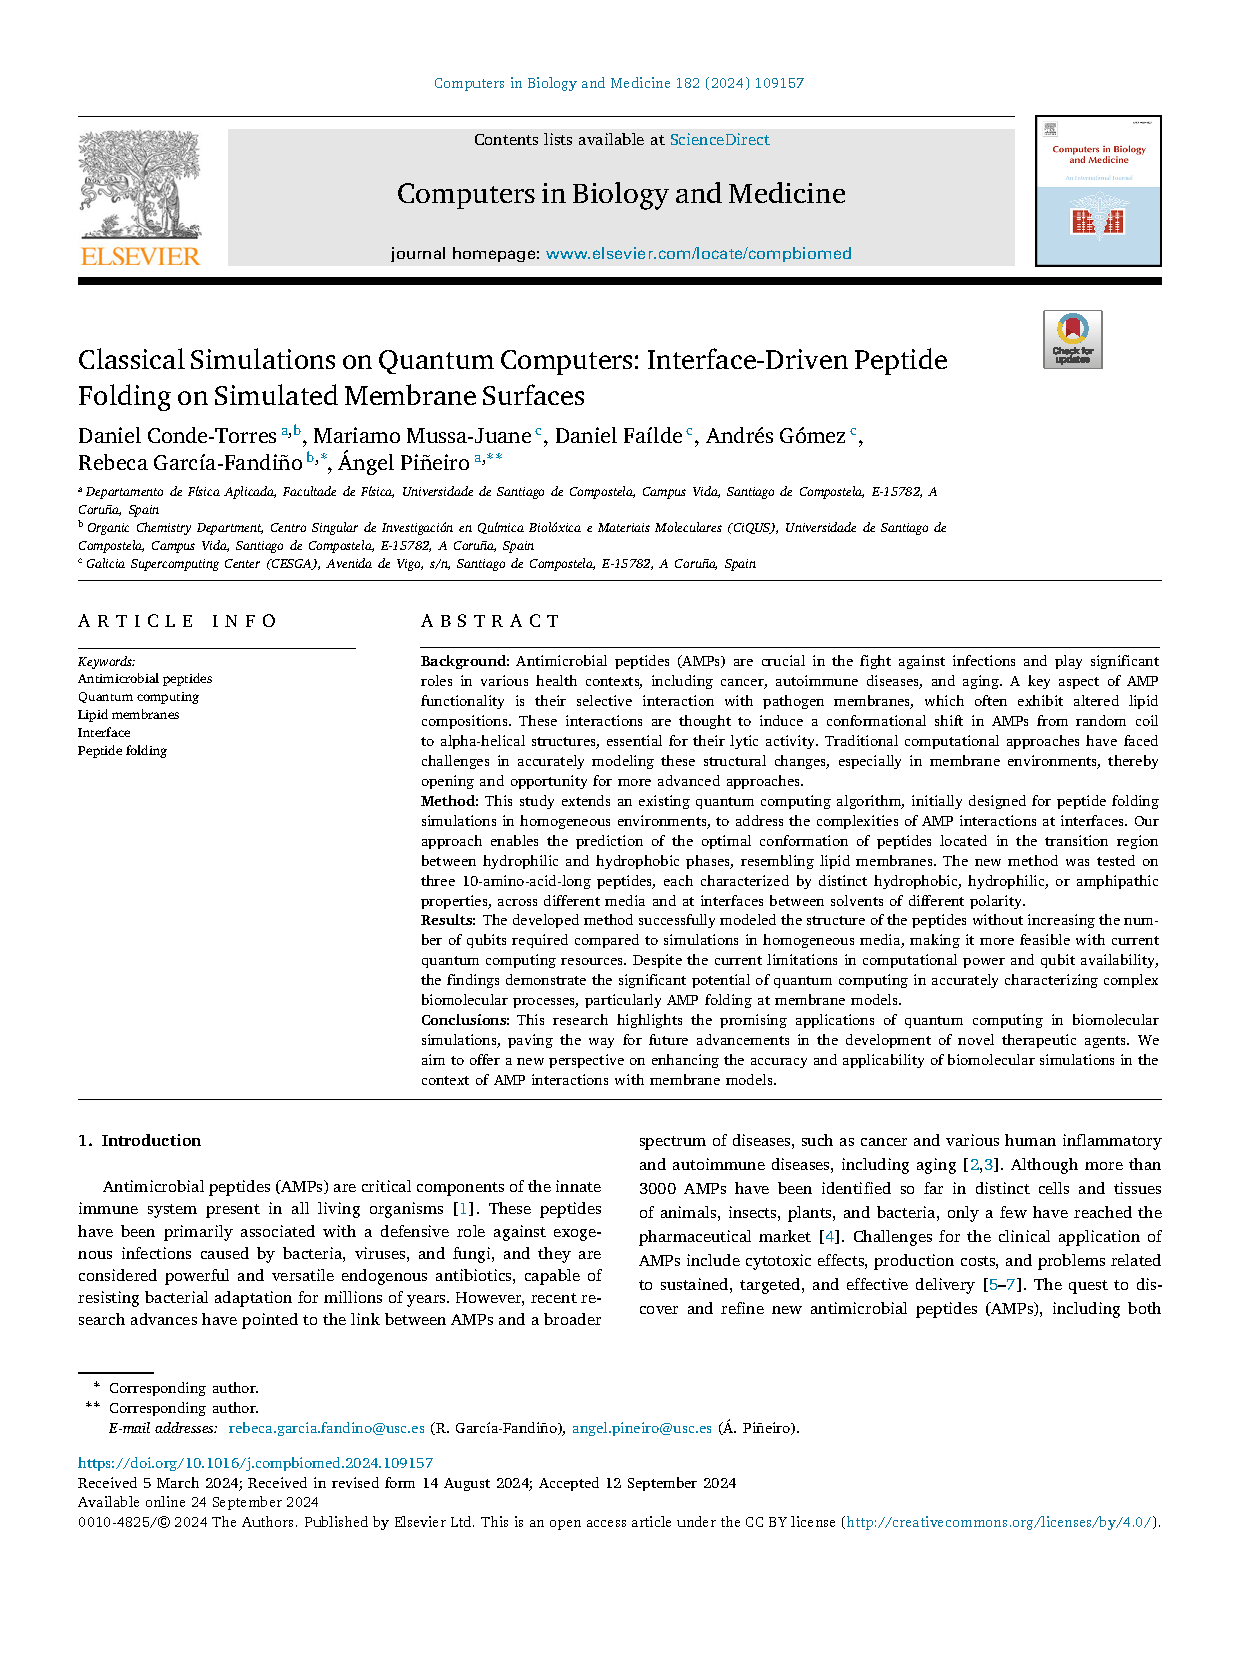
\includegraphics[page=1, width = \linewidth]{Results_Discussion/Papers/Papers_principales/vqe_cesga.pdf}


\includepdf[pages=2-, width = 1.15\linewidth, pagecommand={\thispagestyle{fancy}}]{Results_Discussion/Papers/Papers_principales/vqe_cesga.pdf}
\hypertarget{registro}{}

%% Section 2
% \fakesection{Creating a Database of Cyclic Peptide Molecular Dynamics Results}\label{chap2}
% \chapterquote{GROMACS reminds you: ` `I am rarely happier than when spending an entire day programming my computer to perform automatically a task that it would otherwise take me a good ten seconds to do by hand." (Douglas Adams)}

% \newpage

% \subsection{CYCLOPEpDB: Bridging Molecular Dynamics Simulations and Machine Learning for Predicting Cyclic Peptide-Membrane Interactions.}\label{art:CPDB}

